% Tikz File 'model640.tex'
\documentclass{standalone}

\usepackage{tikz} %Graphics
\usetikzlibrary{shapes.geometric, arrows}
\tikzstyle{title} = [text centered]
\tikzstyle{block} = [rectangle, rounded corners, minimum width=3cm, minimum height=1cm,text centered, draw=black, fill=blue!30]
\tikzstyle{conv} = [rectangle, rounded corners, minimum width=3cm, minimum height=1cm,text centered, draw=black, fill=blue!30]
\tikzstyle{batchnorm} = [rectangle, rounded corners, minimum width=3cm, minimum height=1cm,text centered, draw=black, fill=green!30]
\tikzstyle{relu} = [rectangle, rounded corners, minimum width=3cm, minimum height=1cm,text centered, draw=black, fill=orange!30]
\tikzstyle{maxpool} = [rectangle, rounded corners, minimum width=3cm, minimum height=1cm,text centered, draw=black, fill=red!30]
\tikzstyle{arrow} = [thick,->,>=stealth]

%\usetikzlibrary{...}
\begin{document}
	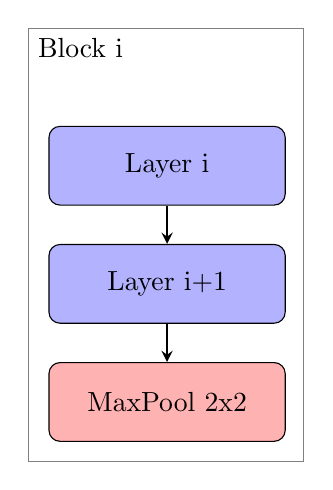
\begin{tikzpicture}[node distance=1.5cm]
		\node (decomp) [title] { Block i };
		\draw [draw=black!50] (decomp.north west) rectangle +(3.5cm, -5.5cm);	
		\node (l1) [conv, below of = decomp, xshift=11mm] {Layer i};
		\node (l2) [conv, below of=l1] {Layer i+1};
		\node (mp) [maxpool, below of=l2] {MaxPool 2x2};
		\draw [arrow] (l1) -- (l2);
		\draw [arrow] (l2) -- (mp);
\end{tikzpicture}
\end{document}
